% Options for packages loaded elsewhere
\PassOptionsToPackage{unicode}{hyperref}
\PassOptionsToPackage{hyphens}{url}
\PassOptionsToPackage{dvipsnames,svgnames,x11names}{xcolor}
%
\documentclass[
  letterpaper,
  DIV=11,
  numbers=noendperiod]{scrartcl}

\usepackage{amsmath,amssymb}
\usepackage{iftex}
\ifPDFTeX
  \usepackage[T1]{fontenc}
  \usepackage[utf8]{inputenc}
  \usepackage{textcomp} % provide euro and other symbols
\else % if luatex or xetex
  \usepackage{unicode-math}
  \defaultfontfeatures{Scale=MatchLowercase}
  \defaultfontfeatures[\rmfamily]{Ligatures=TeX,Scale=1}
\fi
\usepackage{lmodern}
\ifPDFTeX\else  
    % xetex/luatex font selection
\fi
% Use upquote if available, for straight quotes in verbatim environments
\IfFileExists{upquote.sty}{\usepackage{upquote}}{}
\IfFileExists{microtype.sty}{% use microtype if available
  \usepackage[]{microtype}
  \UseMicrotypeSet[protrusion]{basicmath} % disable protrusion for tt fonts
}{}
\makeatletter
\@ifundefined{KOMAClassName}{% if non-KOMA class
  \IfFileExists{parskip.sty}{%
    \usepackage{parskip}
  }{% else
    \setlength{\parindent}{0pt}
    \setlength{\parskip}{6pt plus 2pt minus 1pt}}
}{% if KOMA class
  \KOMAoptions{parskip=half}}
\makeatother
\usepackage{xcolor}
\setlength{\emergencystretch}{3em} % prevent overfull lines
\setcounter{secnumdepth}{-\maxdimen} % remove section numbering
% Make \paragraph and \subparagraph free-standing
\ifx\paragraph\undefined\else
  \let\oldparagraph\paragraph
  \renewcommand{\paragraph}[1]{\oldparagraph{#1}\mbox{}}
\fi
\ifx\subparagraph\undefined\else
  \let\oldsubparagraph\subparagraph
  \renewcommand{\subparagraph}[1]{\oldsubparagraph{#1}\mbox{}}
\fi

\usepackage{color}
\usepackage{fancyvrb}
\newcommand{\VerbBar}{|}
\newcommand{\VERB}{\Verb[commandchars=\\\{\}]}
\DefineVerbatimEnvironment{Highlighting}{Verbatim}{commandchars=\\\{\}}
% Add ',fontsize=\small' for more characters per line
\usepackage{framed}
\definecolor{shadecolor}{RGB}{241,243,245}
\newenvironment{Shaded}{\begin{snugshade}}{\end{snugshade}}
\newcommand{\AlertTok}[1]{\textcolor[rgb]{0.68,0.00,0.00}{#1}}
\newcommand{\AnnotationTok}[1]{\textcolor[rgb]{0.37,0.37,0.37}{#1}}
\newcommand{\AttributeTok}[1]{\textcolor[rgb]{0.40,0.45,0.13}{#1}}
\newcommand{\BaseNTok}[1]{\textcolor[rgb]{0.68,0.00,0.00}{#1}}
\newcommand{\BuiltInTok}[1]{\textcolor[rgb]{0.00,0.23,0.31}{#1}}
\newcommand{\CharTok}[1]{\textcolor[rgb]{0.13,0.47,0.30}{#1}}
\newcommand{\CommentTok}[1]{\textcolor[rgb]{0.37,0.37,0.37}{#1}}
\newcommand{\CommentVarTok}[1]{\textcolor[rgb]{0.37,0.37,0.37}{\textit{#1}}}
\newcommand{\ConstantTok}[1]{\textcolor[rgb]{0.56,0.35,0.01}{#1}}
\newcommand{\ControlFlowTok}[1]{\textcolor[rgb]{0.00,0.23,0.31}{#1}}
\newcommand{\DataTypeTok}[1]{\textcolor[rgb]{0.68,0.00,0.00}{#1}}
\newcommand{\DecValTok}[1]{\textcolor[rgb]{0.68,0.00,0.00}{#1}}
\newcommand{\DocumentationTok}[1]{\textcolor[rgb]{0.37,0.37,0.37}{\textit{#1}}}
\newcommand{\ErrorTok}[1]{\textcolor[rgb]{0.68,0.00,0.00}{#1}}
\newcommand{\ExtensionTok}[1]{\textcolor[rgb]{0.00,0.23,0.31}{#1}}
\newcommand{\FloatTok}[1]{\textcolor[rgb]{0.68,0.00,0.00}{#1}}
\newcommand{\FunctionTok}[1]{\textcolor[rgb]{0.28,0.35,0.67}{#1}}
\newcommand{\ImportTok}[1]{\textcolor[rgb]{0.00,0.46,0.62}{#1}}
\newcommand{\InformationTok}[1]{\textcolor[rgb]{0.37,0.37,0.37}{#1}}
\newcommand{\KeywordTok}[1]{\textcolor[rgb]{0.00,0.23,0.31}{#1}}
\newcommand{\NormalTok}[1]{\textcolor[rgb]{0.00,0.23,0.31}{#1}}
\newcommand{\OperatorTok}[1]{\textcolor[rgb]{0.37,0.37,0.37}{#1}}
\newcommand{\OtherTok}[1]{\textcolor[rgb]{0.00,0.23,0.31}{#1}}
\newcommand{\PreprocessorTok}[1]{\textcolor[rgb]{0.68,0.00,0.00}{#1}}
\newcommand{\RegionMarkerTok}[1]{\textcolor[rgb]{0.00,0.23,0.31}{#1}}
\newcommand{\SpecialCharTok}[1]{\textcolor[rgb]{0.37,0.37,0.37}{#1}}
\newcommand{\SpecialStringTok}[1]{\textcolor[rgb]{0.13,0.47,0.30}{#1}}
\newcommand{\StringTok}[1]{\textcolor[rgb]{0.13,0.47,0.30}{#1}}
\newcommand{\VariableTok}[1]{\textcolor[rgb]{0.07,0.07,0.07}{#1}}
\newcommand{\VerbatimStringTok}[1]{\textcolor[rgb]{0.13,0.47,0.30}{#1}}
\newcommand{\WarningTok}[1]{\textcolor[rgb]{0.37,0.37,0.37}{\textit{#1}}}

\providecommand{\tightlist}{%
  \setlength{\itemsep}{0pt}\setlength{\parskip}{0pt}}\usepackage{longtable,booktabs,array}
\usepackage{calc} % for calculating minipage widths
% Correct order of tables after \paragraph or \subparagraph
\usepackage{etoolbox}
\makeatletter
\patchcmd\longtable{\par}{\if@noskipsec\mbox{}\fi\par}{}{}
\makeatother
% Allow footnotes in longtable head/foot
\IfFileExists{footnotehyper.sty}{\usepackage{footnotehyper}}{\usepackage{footnote}}
\makesavenoteenv{longtable}
\usepackage{graphicx}
\makeatletter
\def\maxwidth{\ifdim\Gin@nat@width>\linewidth\linewidth\else\Gin@nat@width\fi}
\def\maxheight{\ifdim\Gin@nat@height>\textheight\textheight\else\Gin@nat@height\fi}
\makeatother
% Scale images if necessary, so that they will not overflow the page
% margins by default, and it is still possible to overwrite the defaults
% using explicit options in \includegraphics[width, height, ...]{}
\setkeys{Gin}{width=\maxwidth,height=\maxheight,keepaspectratio}
% Set default figure placement to htbp
\makeatletter
\def\fps@figure{htbp}
\makeatother

\KOMAoption{captions}{tableheading}
\makeatletter
\makeatother
\makeatletter
\makeatother
\makeatletter
\@ifpackageloaded{caption}{}{\usepackage{caption}}
\AtBeginDocument{%
\ifdefined\contentsname
  \renewcommand*\contentsname{Table of contents}
\else
  \newcommand\contentsname{Table of contents}
\fi
\ifdefined\listfigurename
  \renewcommand*\listfigurename{List of Figures}
\else
  \newcommand\listfigurename{List of Figures}
\fi
\ifdefined\listtablename
  \renewcommand*\listtablename{List of Tables}
\else
  \newcommand\listtablename{List of Tables}
\fi
\ifdefined\figurename
  \renewcommand*\figurename{Figure}
\else
  \newcommand\figurename{Figure}
\fi
\ifdefined\tablename
  \renewcommand*\tablename{Table}
\else
  \newcommand\tablename{Table}
\fi
}
\@ifpackageloaded{float}{}{\usepackage{float}}
\floatstyle{ruled}
\@ifundefined{c@chapter}{\newfloat{codelisting}{h}{lop}}{\newfloat{codelisting}{h}{lop}[chapter]}
\floatname{codelisting}{Listing}
\newcommand*\listoflistings{\listof{codelisting}{List of Listings}}
\makeatother
\makeatletter
\@ifpackageloaded{caption}{}{\usepackage{caption}}
\@ifpackageloaded{subcaption}{}{\usepackage{subcaption}}
\makeatother
\makeatletter
\@ifpackageloaded{tcolorbox}{}{\usepackage[skins,breakable]{tcolorbox}}
\makeatother
\makeatletter
\@ifundefined{shadecolor}{\definecolor{shadecolor}{rgb}{.97, .97, .97}}
\makeatother
\makeatletter
\makeatother
\makeatletter
\makeatother
\ifLuaTeX
  \usepackage{selnolig}  % disable illegal ligatures
\fi
\IfFileExists{bookmark.sty}{\usepackage{bookmark}}{\usepackage{hyperref}}
\IfFileExists{xurl.sty}{\usepackage{xurl}}{} % add URL line breaks if available
\urlstyle{same} % disable monospaced font for URLs
\hypersetup{
  pdftitle={travail\_session\_akyildiz},
  pdfauthor={Egemen Akyildiz},
  colorlinks=true,
  linkcolor={blue},
  filecolor={Maroon},
  citecolor={Blue},
  urlcolor={Blue},
  pdfcreator={LaTeX via pandoc}}

\title{travail\_session\_akyildiz}
\author{Egemen Akyildiz}
\date{}

\begin{document}
\maketitle
\ifdefined\Shaded\renewenvironment{Shaded}{\begin{tcolorbox}[breakable, interior hidden, borderline west={3pt}{0pt}{shadecolor}, frame hidden, sharp corners, enhanced, boxrule=0pt]}{\end{tcolorbox}}\fi

\hypertarget{annexe}{%
\section{annexe}\label{annexe}}

\begin{Shaded}
\begin{Highlighting}[]
\FunctionTok{library}\NormalTok{(haven)}
\end{Highlighting}
\end{Shaded}

\begin{verbatim}
Warning: package 'haven' was built under R version 4.3.3
\end{verbatim}

\begin{Shaded}
\begin{Highlighting}[]
\NormalTok{data }\OtherTok{\textless{}{-}} \FunctionTok{read\_sav}\NormalTok{(}\StringTok{"ess2022.sav"}\NormalTok{)}
\FunctionTok{head}\NormalTok{(data)}
\end{Highlighting}
\end{Shaded}

\begin{verbatim}
# A tibble: 6 x 258
  UID_fes2 fes2_EE22_Q01A           fes2_EE22_Q01B fes2_EE22_Q02A fes2_EE22_Q02B
     <dbl> <dbl+lbl>                <dbl+lbl>      <dbl+lbl>      <dbl+lbl>     
1      917 14 [Les déficits public~  6 [L’Union e~ 10 [La relanc~  6 [L’Union e~
2        3  1 [Le système de prote~  4 [L’immigra~ 12 [Le pouvoi~  7 [La démocr~
3     1040  4 [L’immigration]        6 [L’Union e~  4 [L’immigra~  6 [L’Union e~
4      295  2 [L’éducation et la f~  1 [Le systèm~  1 [Le systèm~  2 [L’éducati~
5       71  8 [La protection de l’~ 16 [Les inéga~ 10 [La relanc~  1 [Le systèm~
6      146  1 [Le système de prote~ 10 [La relanc~  5 [L’insécur~ 12 [Le pouvoi~
# i 253 more variables: fes2_EE22_Q03_A_P <dbl+lbl>,
#   fes2_EE22_Q03_B_P <dbl+lbl>, fes2_EE22_Q05_1 <dbl+lbl>,
#   fes2_EE22_Q05_2 <dbl+lbl>, fes2_EE22_Q05_3 <dbl+lbl>,
#   fes2_EE22_Q05_4 <dbl+lbl>, fes2_EE22_Q05_5 <dbl+lbl>,
#   fes2_EE22_Q08_1 <dbl+lbl>, fes2_EE22_Q08_2 <dbl+lbl>,
#   fes2_EE22_Q08_3 <dbl+lbl>, fes2_EE22_Q08_4 <dbl+lbl>,
#   fes2_EE22_Q08_5 <dbl+lbl>, fes2_EE22_Q08_6 <dbl+lbl>, ...
\end{verbatim}

\begin{Shaded}
\begin{Highlighting}[]
\FunctionTok{library}\NormalTok{(ggplot2)}
\end{Highlighting}
\end{Shaded}

\begin{verbatim}
Warning: package 'ggplot2' was built under R version 4.3.3
\end{verbatim}

\begin{Shaded}
\begin{Highlighting}[]
\FunctionTok{library}\NormalTok{(tidyverse)}
\end{Highlighting}
\end{Shaded}

\begin{verbatim}
Warning: package 'tidyverse' was built under R version 4.3.2
\end{verbatim}

\begin{verbatim}
Warning: package 'tidyr' was built under R version 4.3.2
\end{verbatim}

\begin{verbatim}
Warning: package 'readr' was built under R version 4.3.2
\end{verbatim}

\begin{verbatim}
Warning: package 'purrr' was built under R version 4.3.2
\end{verbatim}

\begin{verbatim}
Warning: package 'dplyr' was built under R version 4.3.2
\end{verbatim}

\begin{verbatim}
Warning: package 'stringr' was built under R version 4.3.2
\end{verbatim}

\begin{verbatim}
Warning: package 'forcats' was built under R version 4.3.2
\end{verbatim}

\begin{verbatim}
Warning: package 'lubridate' was built under R version 4.3.2
\end{verbatim}

\begin{verbatim}
-- Attaching core tidyverse packages ------------------------ tidyverse 2.0.0 --
v dplyr     1.1.4     v readr     2.1.5
v forcats   1.0.0     v stringr   1.5.1
v lubridate 1.9.3     v tibble    3.2.1
v purrr     1.0.2     v tidyr     1.3.1
-- Conflicts ------------------------------------------ tidyverse_conflicts() --
x dplyr::filter() masks stats::filter()
x dplyr::lag()    masks stats::lag()
i Use the conflicted package (<http://conflicted.r-lib.org/>) to force all conflicts to become errors
\end{verbatim}

\begin{Shaded}
\begin{Highlighting}[]
\NormalTok{data\_nettoye }\OtherTok{\textless{}{-}} \FunctionTok{select}\NormalTok{(data, eayy\_a1, fes2\_EE22\_Q17, eayy\_a2a\_rec2, eayy\_b18\_rec, fes2\_EE22\_Q10C, fes2\_EE22\_Q10E, fes2\_EE22\_Q01A, fes2\_EE22\_Q01B, eayy\_h\_teo1, eayy\_i2, eayy\_f9, eayy\_e5)}


\NormalTok{data\_super\_nettoye }\OtherTok{\textless{}{-}} \FunctionTok{rename}\NormalTok{(data\_nettoye, }
                             \AttributeTok{Sexe =}\NormalTok{ eayy\_a1,}
                             \AttributeTok{Remplacement =}\NormalTok{ fes2\_EE22\_Q17,}
                             \AttributeTok{Age =}\NormalTok{ eayy\_a2a\_rec2,}
                             \AttributeTok{Diplome =}\NormalTok{ eayy\_b18\_rec,}
                             \AttributeTok{Vote\_Zemmour =}\NormalTok{ fes2\_EE22\_Q10C,}
                             \AttributeTok{Vote\_Le\_Pen =}\NormalTok{ fes2\_EE22\_Q10E,}
                             \AttributeTok{Premiere\_thematique =}\NormalTok{ fes2\_EE22\_Q01A,}
                             \AttributeTok{Deuxieme\_thematique =}\NormalTok{ fes2\_EE22\_Q01B,}
                             \AttributeTok{Religiosite =}\NormalTok{ eayy\_h\_teo1,}
                             \AttributeTok{Fonctionnement\_de\_la\_democratie =}\NormalTok{ eayy\_i2,}
                             \AttributeTok{Confiance\_aux\_autres =}\NormalTok{ eayy\_f9,}
                             \AttributeTok{Situation\_financiere =}\NormalTok{ eayy\_e5)}


\NormalTok{data\_super\_nettoye2 }\OtherTok{\textless{}{-}} \FunctionTok{na.omit}\NormalTok{(data\_super\_nettoye)}
\end{Highlighting}
\end{Shaded}

\hypertarget{introduction-probluxe9matique-et-question}{%
\subsection{Introduction, problématique et
question}\label{introduction-probluxe9matique-et-question}}

L\textquotesingle objet de cette étude est de découvrir les
caractéristiques des électeurs d\textquotesingle extrême droite. Quelles
sont ces caractéristiques? Notre hypothèse est que le Rassemblement
National n\textquotesingle est plus un parti d\textquotesingle extrême
droite, ou que seule une minorité de sa base électorale
l\textquotesingle est, que Reconquête est le nouveau parti
d\textquotesingle extrême droite en plus de la base extrême droite
restante du Rassemblement National et que les caractéristiques
principales d\textquotesingle un électeur d\textquotesingle extrême
droite est un revenu faible, un manque de confiance aux autres et une
déception de la démocratie en France. Nous assignons
l\textquotesingle électeur de l\textquotesingle extrême à une réponse
favorable ou un peu favorable à la question d\textquotesingle une
croyance au grand remplacement. L'élection présidentielle de 2022 en
France a été marquée par une polarisation politique intense et des
débats passionnés sur les idéologies et les orientations des électeurs.
Malgré~la guerre en Ukraine, le début de la course présidentielle avait
marqué un profond ancrage de sujets reliés à l\textquotesingle extrême
droite française, incarnée avant tout par Éric Zemmour et son nouveau
parti «~Reconquête~». L\textquotesingle ancienne figure phare du camp
politique de l\textquotesingle extrême droite est Marine Le Pen mais
l\textquotesingle arrivée du journaliste dans la course à la présidence
a changé les paramètres habituels de la politique française.

Nous devrions tout d\textquotesingle abord mettre une chose au clair.
Qu\textquotesingle est-ce que nous entendons par «~extrême droite~»? Le
terme est extrêmement vague et très peu limité. En général, les partis
d\textquotesingle extrême gauche ou droite sont par définition
minoritaires. Pourrions-nous alors prendre le Rassemblement National
comme un parti d\textquotesingle extrême droite alors que presque la
moitié des français vote pour celui-ci. Ceci ne serait pas utile, notre
objectif est de décrire une partie spécifique de la population qui doit,
pour l\textquotesingle utilité de cet exercice, être minoritaire afin
d\textquotesingle avoir des caractéristiques spécifiques.

Le spectre gauche-droite est comme le qualificatif
l\textquotesingle indique un spectre. Ceci veut dire
qu\textquotesingle il y a un mouvement à l\textquotesingle intérieur de
ce spectre. Le clivage bouge en même temps que les orientations
idéologiques des partis bougent (Quinchon-Caudal 2021).
L\textquotesingle extrême droite de hier peut être la droite
d\textquotesingle aujourd\textquotesingle hui (Quinchon-Caudal 2021).
Ceci irait avec le concept du « Radical Right Gender Gap » qui soutient
que le fait que la candidate phare du Rassemblement National soit une
femme fait en sorte que les femmes auraient tendances à voter plus pour
des partis plus à droite comme celui-ci (Amengay et al 2017).
L\textquotesingle arrivée de ces nouvelles électrices au Rassemblement
National a sûrement eu un effet d\textquotesingle adoucissement des
discours de ce parti et un penchant plus à gauche sur certains sujets.
Ceci nous semble une des explications plausibles pour cet écart et les
changements récents du Parti.

De plus, nous allons aussi nous focaliser sur une question clé à
laquelle les répondants du sondage que nous allons utiliser ont eu à
répondre. Celle-ci est la croyance à la théorie du «~grand
remplacement~». Un trait très prégnant d\textquotesingle une adhérence à
l\textquotesingle extrême droite en France et en Europe est une réponse
affirmative à cette question (Ivaldi 2014). Cette théorie soutient
qu\textquotesingle il existe un projet d\textquotesingle une immigration
massive venant du sud majoritairement musulman pour remplacer la
population locale. Tout ceci orchestré par une élite politique.

\hypertarget{raisons-motivants-la-recherche}{%
\subsection{Raisons motivants la
recherche}\label{raisons-motivants-la-recherche}}

Avec la montée des populismes en Europe, surtout de droite,
l\textquotesingle arrivée massive de migrants du sud, la défaite
économique des classes ouvrières à cause de la globalisation et la
baisse du niveau de vie des classes moyennes, nous nous inquiétons pour
la stabilité de cette partie du monde. Les souvenirs des années 30 et 40
sont toujours vivants mais nous avons l\textquotesingle impression que
ceux-ci s\textquotesingle estompent au fur et à mesure que les années
passent. En dehors des parallèles historiques aisément réalisables, nous
nous inquiétons aussi des programmes futurs des partis politiques. Nous
partons de la supposition que les opinions des électeurs créent les
programmes politiques, dans la logique de la demande qui cause la
production. Tout cela n\textquotesingle est pas spécifiquement européen,
il y a une baisse de la démocratie, même de l\textquotesingle importance
apporté à celle-ci par les populations qui y vivent. Toutefois, assez
ironiquement l\textquotesingle amour de la démocratie est en croissance
en Afrique qui elle n\textquotesingle a que très peu de régime
démocratique (Ghana, Botswana, Mauritius).

\hypertarget{les-donnuxe9es}{%
\subsection{Les données}\label{les-donnuxe9es}}

Pour répondre à nos questions de recherche, nous allons utiliser la base
de données de la «~french electoral study~» de 2022. Cette base de
données est composée des réponses reçues à un sondage donné aux
électeurs français de l\textquotesingle élection présidentielle de 2022.
Le nombre de répondants est de 1614. Ceux-ci sont les 84,7\% des 1905
invités à répondre à l\textquotesingle enquête électorale. Ils sont tous
issues de la France Métropolitaine hors Corse. Ceci est important car
par exemple les électeurs du Rassemblement National de Mayotte sont
exclus, ceux-ci sont un cas à part dû à la proximité des Comores et du
flux migratoire important qui cause ce vote.

Notre base de données est aussi composée des variables auxquelles nos
répondants ont répondu de «~l\textquotesingle Enquête annuelle~». Les
variables se comptent au nombre de 258. Les répondants ont été choisis
aléatoirement. Elles sont toutes ordinales en dehors des variables
dichotomiques comme le sexe. Elles sont des questions sur les
caractéristiques socio-économiques, démographiques, le sexe,
l\textquotesingle âge, le statut familial et marital, le nombre
d\textquotesingle enfants et encore plus. Les questions plus axées sur
la politique sont en première partie celles qui portent sur les
thématiques les plus importantes et les autres sur les candidats, leur
qualification gauche-droite et la préférence du répondant pour
l\textquotesingle un deux. Les variables qui nous intéressent sont, pour
la partie politique, les questions reliées à Marine Le Pen et Zemmour,
la démocratie, et la fameuse question du grand remplacement. Pour les
caractéristiques socio-démographiques comme le sexe, le niveau de vie
(ou la perception du niveau de vie) vont être utilisées avec les
variables politiques. Il est important de noter dès le début que 53,2\%
des répondants sont des femmes, 46,8\% des hommes. C\textquotesingle est
pour cela que quand nous utiliserons la variable sexe, nous allons
prendre en compte cette légère différence. ~

\hypertarget{analyse-et-ruxe9sultats}{%
\subsection{Analyse et résultats}\label{analyse-et-ruxe9sultats}}

Puisque nous ne comptons pas utiliser toutes les variables de notre base
de données, nous avons sélectionner (avec la fonction select()) celles
qui nous intéressent le plus~: le sexe, la croyance au grand
remplacement, l\textquotesingle intention de vote pour Marine Le Pen et
Zemmour, la confiance aux autres, la vision du fonctionnement de la
démocratie et la situation financière des répondants.

Ensuite, nous les avons renommées pour que nous puissions les manipuler
plus facilement avec la fonction rename(). Et nous avons éliminé les
lignes avec des variables manquantes grâce à la fonction na.omit(). De
plus nous avons factorisé la variable «~Sexe~» pour que nous puissions
l\textquotesingle utiliser avec des barres groupées.

Tout d\textquotesingle abord, nous allons vérifier la proportion
d\textquotesingle hommes et de femmes qui croient en cette théorie.
Comme nous pouvons le constater, le nombre de femmes est relativement
moins élevée que celui des hommes. En terme général, la majorité des
participants n\textquotesingle y croit pas et une part non-négligeable
des femmes ont répondu qu\textquotesingle elles ne savent pas si un tel
projet existe ou pas. Une théorie intéressante est celle de
l\textquotesingle anthropologue Emmanuel Todd. Celui-ci avance que les
femmes sont moins racistes que les hommes en utilisant des données
statistiques américaines (Todd 2021). Les femmes blanches sont 5 fois
plus susceptibles de se marier à un homme noir que
l\textquotesingle inverse. Ceci est dû selon lui à deux valeurs
fondamentales qui séparent les deux sexes. Les femmes sont altruistes et
individualistes, les hommes égoïstes et collectivistes.
L\textquotesingle aspect plus raciste des hommes viendraient de leur
tendance au collectif, au groupe (Todd 2021). ~Les hommes voient le
monde en groupe, et rejettent les autres groupes par égoïsme, tandis que
les femmes voient beaucoup plus les individus en tant que tels et sont
plus aptes à ne pas penser qu\textquotesingle à elle-même (Todd 2021).

\begin{Shaded}
\begin{Highlighting}[]
\FunctionTok{ggplot}\NormalTok{(data\_super\_nettoye2, }\FunctionTok{aes}\NormalTok{(}\AttributeTok{x =}\NormalTok{ Remplacement, }\AttributeTok{fill =}\NormalTok{ Sexe)) }\SpecialCharTok{+}
  \FunctionTok{geom\_bar}\NormalTok{(}\AttributeTok{position =} \StringTok{"dodge"}\NormalTok{) }\SpecialCharTok{+}
    \FunctionTok{labs}\NormalTok{(}\AttributeTok{x =} \StringTok{"Croyance au grand remplacement"}\NormalTok{, }\AttributeTok{y =} \StringTok{"Fréquence"}\NormalTok{, }\AttributeTok{fill =} \StringTok{"Sexe"}\NormalTok{) }\SpecialCharTok{+}
   \FunctionTok{scale\_x\_discrete}\NormalTok{(}\AttributeTok{labels =} \FunctionTok{c}\NormalTok{(}\StringTok{"Oui"}\NormalTok{, }\StringTok{"Probablement"}\NormalTok{, }\StringTok{"Probablement pas"}\NormalTok{, }\StringTok{"Non"}\NormalTok{, }\StringTok{"Je ne sais pas"}\NormalTok{)) }\SpecialCharTok{+}
  \FunctionTok{scale\_fill\_manual}\NormalTok{(}\AttributeTok{labels =} \FunctionTok{c}\NormalTok{(}\StringTok{"Homme"}\NormalTok{, }\StringTok{"Femme"}\NormalTok{), }\AttributeTok{values =} \FunctionTok{c}\NormalTok{(}\StringTok{"1"} \OtherTok{=} \StringTok{"blue"}\NormalTok{, }\StringTok{"2"} \OtherTok{=} \StringTok{"red"}\NormalTok{)) }\SpecialCharTok{+}
  \FunctionTok{ggtitle}\NormalTok{(}\StringTok{"Croyance au grand remplacement par sexe"}\NormalTok{) }\SpecialCharTok{+}
   \FunctionTok{theme}\NormalTok{(}\AttributeTok{plot.title =} \FunctionTok{element\_text}\NormalTok{(}\AttributeTok{face =} \StringTok{"bold"}\NormalTok{, }\AttributeTok{family =} \StringTok{"Arial"}\NormalTok{)) }\SpecialCharTok{+}
  \FunctionTok{theme\_minimal}\NormalTok{()}
\end{Highlighting}
\end{Shaded}

\begin{verbatim}
Warning: The following aesthetics were dropped during statistical transformation: fill.
i This can happen when ggplot fails to infer the correct grouping structure in
  the data.
i Did you forget to specify a `group` aesthetic or to convert a numerical
  variable into a factor?
\end{verbatim}

\begin{verbatim}
Warning: No shared levels found between `names(values)` of the manual scale and the
data's fill values.
\end{verbatim}

\begin{figure}[H]

{\centering 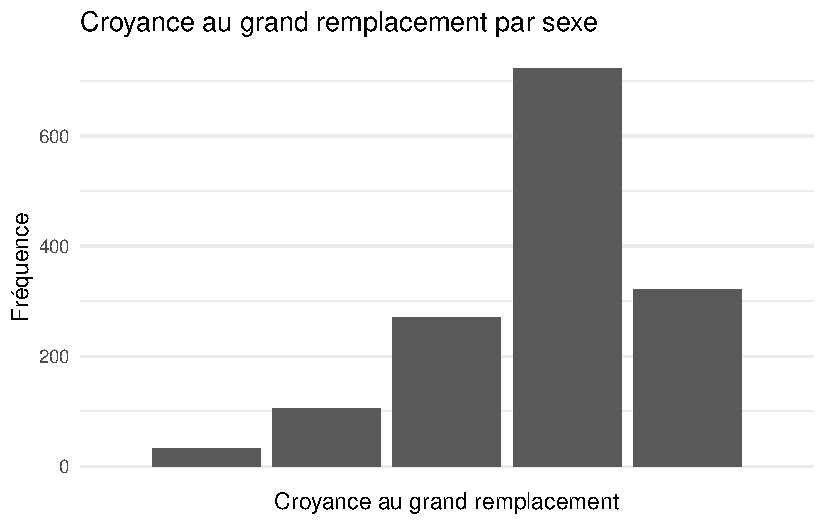
\includegraphics{travail_session_Akyildiz_files/figure-pdf/unnamed-chunk-3-1.pdf}

}

\end{figure}

Dans les prochains graphiques nous allons vérifier la présence des
croyants au grand remplacement au sein des potentiels électeurs de
Zemmour et Le Pen.

\begin{Shaded}
\begin{Highlighting}[]
\FunctionTok{ggplot}\NormalTok{(data\_super\_nettoye2, }\FunctionTok{aes}\NormalTok{(}\AttributeTok{x =} \FunctionTok{factor}\NormalTok{(Remplacement), }\AttributeTok{fill =} \FunctionTok{factor}\NormalTok{(Vote\_Zemmour))) }\SpecialCharTok{+}
  \FunctionTok{geom\_bar}\NormalTok{(}\AttributeTok{position =} \StringTok{"stack"}\NormalTok{) }\SpecialCharTok{+}
  \FunctionTok{labs}\NormalTok{(}\AttributeTok{x =} \StringTok{"Croyance au grand remplacement"}\NormalTok{, }\AttributeTok{y =} \StringTok{"Fréquence"}\NormalTok{, }\AttributeTok{fill =} \StringTok{"Vote pour Zemmour"}\NormalTok{, }\AttributeTok{title =} \StringTok{"Le vote zemmouriste et la croyance au grand remplacement"}\NormalTok{) }\SpecialCharTok{+}
  \FunctionTok{scale\_x\_discrete}\NormalTok{(}\AttributeTok{labels =} \FunctionTok{c}\NormalTok{(}\StringTok{"Oui"}\NormalTok{, }\StringTok{"Probablement"}\NormalTok{, }\StringTok{"Probablement pas"}\NormalTok{, }\StringTok{"Non"}\NormalTok{, }\StringTok{"Je ne sais pas"}\NormalTok{)) }\SpecialCharTok{+}
  \FunctionTok{theme\_minimal}\NormalTok{()}
\end{Highlighting}
\end{Shaded}

\begin{figure}[H]

{\centering 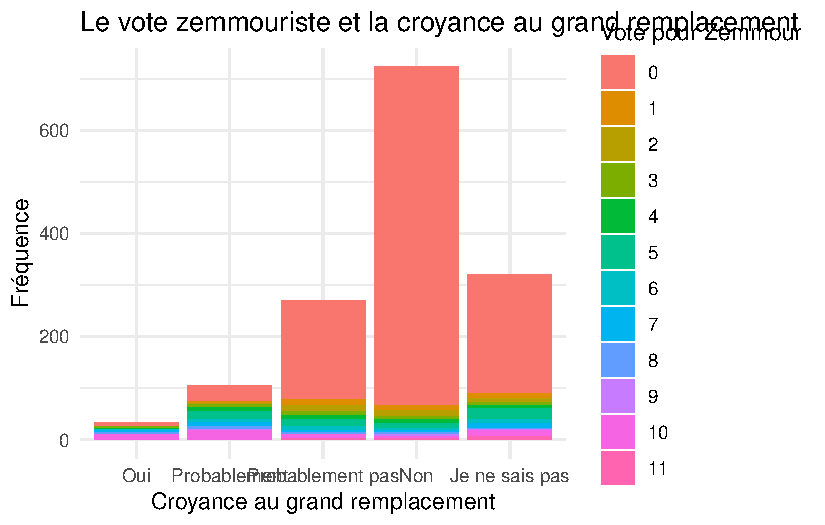
\includegraphics{travail_session_Akyildiz_files/figure-pdf/unnamed-chunk-4-1.pdf}

}

\end{figure}

\begin{Shaded}
\begin{Highlighting}[]
\FunctionTok{ggplot}\NormalTok{(data\_super\_nettoye2, }\FunctionTok{aes}\NormalTok{(}\AttributeTok{x =} \FunctionTok{factor}\NormalTok{(Remplacement), }\AttributeTok{fill =} \FunctionTok{factor}\NormalTok{(Vote\_Le\_Pen))) }\SpecialCharTok{+}
  \FunctionTok{geom\_bar}\NormalTok{(}\AttributeTok{position =} \StringTok{"stack"}\NormalTok{) }\SpecialCharTok{+}
  \FunctionTok{labs}\NormalTok{(}\AttributeTok{x =} \StringTok{"Croyance au grand remplacement"}\NormalTok{, }\AttributeTok{y =} \StringTok{"Fréquence"}\NormalTok{, }\AttributeTok{fill =} \StringTok{"Vote pour Le Pen"}\NormalTok{, }\AttributeTok{title =} \StringTok{"Le vote LePéniste et la croyance au grand remplacement"}\NormalTok{) }\SpecialCharTok{+}
  \FunctionTok{scale\_x\_discrete}\NormalTok{(}\AttributeTok{labels =} \FunctionTok{c}\NormalTok{(}\StringTok{"Oui"}\NormalTok{, }\StringTok{"Probablement"}\NormalTok{, }\StringTok{"Probablement pas"}\NormalTok{, }\StringTok{"Non"}\NormalTok{, }\StringTok{"Je ne sais pas"}\NormalTok{)) }\SpecialCharTok{+}
  \FunctionTok{theme\_minimal}\NormalTok{()}
\end{Highlighting}
\end{Shaded}

\begin{figure}[H]

{\centering 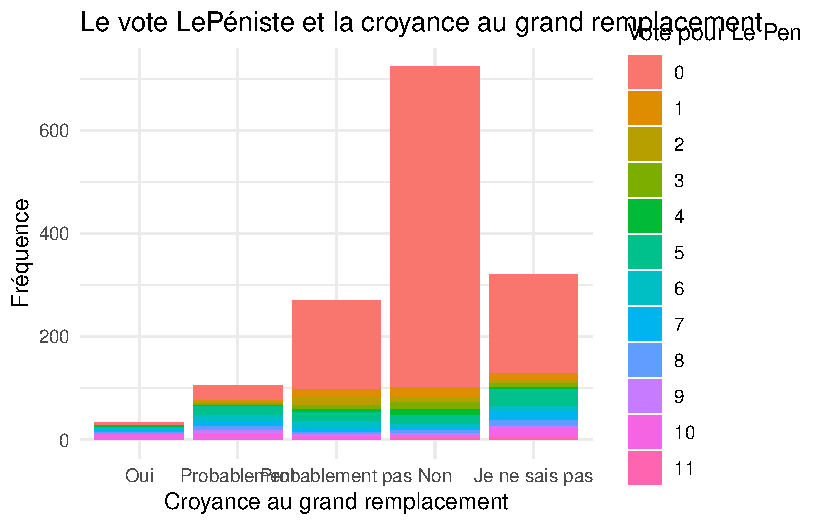
\includegraphics{travail_session_Akyildiz_files/figure-pdf/unnamed-chunk-5-1.pdf}

}

\end{figure}

Nous pouvons très nettement voir qu\textquotesingle à part quelques cas
très isolés, les électeurs de ces deux candidats y croient. En plus,
ceux qui n\textquotesingle y croit certainement pas sont pratiquement
absents. Les gens qui ne croient pas en cette théorie sont absents de
leur électorat. Les deux graphiques sont quasiment identiques.
N\textquotesingle étant pas sûr des résultats après la choquante
ressemblance, nous avons vérifié ceux-ci dans le document associé à la
base de données et confirmé qu\textquotesingle en effet ceux-ci sont
extrêmement similaires. Les deux électorats semblent être tous deux
extrêmement unis sur la question migratoire à cause de cette croyance ou
semi-croyance à une théorie du complot.

Maintenant, intéressons-nous aux autres variables qui montreraient les
caractéristiques des électeurs d\textquotesingle extrême droite. Ceux-ci
sont-ils des gens qui voient le fonctionnement de la démocratie en
France de manière positive, ont confiance aux autres, et ont une
situation financière correcte ?

\begin{Shaded}
\begin{Highlighting}[]
\FunctionTok{ggplot}\NormalTok{(data\_super\_nettoye2, }\FunctionTok{aes}\NormalTok{(}\AttributeTok{x =} \FunctionTok{factor}\NormalTok{(Remplacement), }\AttributeTok{fill =} \FunctionTok{factor}\NormalTok{(Situation\_financiere))) }\SpecialCharTok{+}
  \FunctionTok{geom\_bar}\NormalTok{(}\AttributeTok{position =} \StringTok{"stack"}\NormalTok{) }\SpecialCharTok{+}
  \FunctionTok{labs}\NormalTok{(}\AttributeTok{x =} \StringTok{"Croyance au grand remplacement"}\NormalTok{, }\AttributeTok{y =} \StringTok{"Fréquence"}\NormalTok{, }\AttributeTok{fill =} \StringTok{"Situation financière"}\NormalTok{, }\AttributeTok{title =} \StringTok{"Le niveau de vie et la croyance au grand remplacement"}\NormalTok{) }\SpecialCharTok{+}
  \FunctionTok{scale\_x\_discrete}\NormalTok{(}\AttributeTok{labels =} \FunctionTok{c}\NormalTok{(}\StringTok{"Oui"}\NormalTok{, }\StringTok{"Probablement"}\NormalTok{, }\StringTok{"Probablement pas"}\NormalTok{, }\StringTok{"Non"}\NormalTok{, }\StringTok{"Je ne sais pas"}\NormalTok{)) }\SpecialCharTok{+}
  \FunctionTok{scale\_fill\_discrete}\NormalTok{(}\AttributeTok{labels =} \FunctionTok{c}\NormalTok{(}\StringTok{"Pas possible sans dette"}\NormalTok{, }\StringTok{"Difficile"}\NormalTok{, }\StringTok{"Très juste"}\NormalTok{, }\StringTok{"Passable"}\NormalTok{, }\StringTok{"Ça va"}\NormalTok{, }\StringTok{"À l\textquotesingle{}aise"}\NormalTok{, }\StringTok{"Très à l\textquotesingle{}aise"}\NormalTok{)) }\SpecialCharTok{+}
  \FunctionTok{theme\_minimal}\NormalTok{()}
\end{Highlighting}
\end{Shaded}

\begin{figure}[H]

{\centering 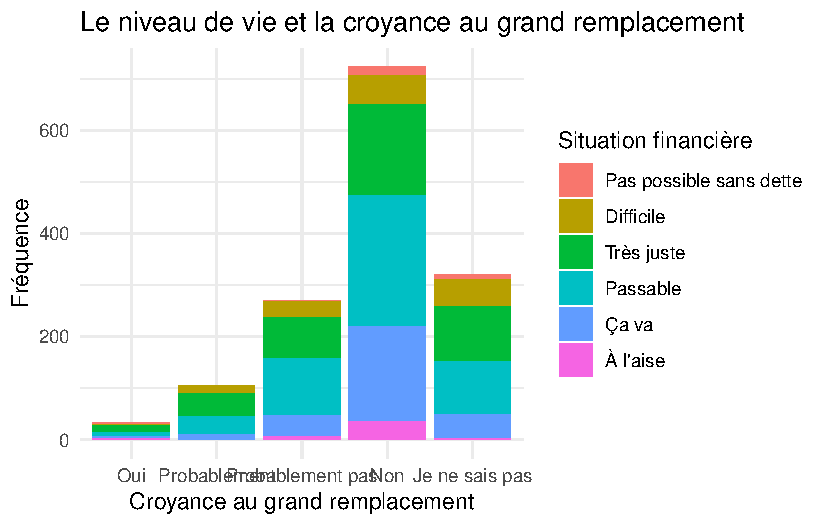
\includegraphics{travail_session_Akyildiz_files/figure-pdf/unnamed-chunk-6-1.pdf}

}

\end{figure}

Les résultats ne sont pas très choquants. Les gens qui ont le meilleur
niveau de vie par aisance financière sont ceux qui ne croient pas au
grand remplacement. Par contre, il n'y en a pratiquement pas pour ceux
qui croient en la théorie ou presque. Assez étrangement, certains qui
ont répondu certainement oui à la réponse du grand remplacement ont un
niveau de vie à l'aise tandis que ceux qui n'y croient pas totalement
n'ont presque aucun membre à l'aise. Aurions-nous trouver une trace
d'une bourgeoisie déclassé? Ceci rentre dans le contexte de
globalisation qui engendre des classes moyennes et ouvrières largement
perdantes face à la concurrence des États étrangers (Goodliffe 2012).
Celles-ci mettraient la faute sur les autres États qui en plus
d\textquotesingle obtenir les usines et les métiers traditionnels des
locaux, envoient des ressortissants les prendre chez eux-mêmes
(Goodliffe 2012). Mais une partie de la bourgeoisie peut elle aussi
perdre sa place dans la globalisation. Proportionnellement parlant, la
part des gens en difficulté est plus élevée pour ceux qui y croient.
Encore une autre hypothèse confirmée.

\begin{Shaded}
\begin{Highlighting}[]
\FunctionTok{ggplot}\NormalTok{(data\_super\_nettoye2, }\FunctionTok{aes}\NormalTok{(}\AttributeTok{x =} \FunctionTok{factor}\NormalTok{(Remplacement), }\AttributeTok{fill =} \FunctionTok{factor}\NormalTok{(Confiance\_aux\_autres))) }\SpecialCharTok{+}
  \FunctionTok{geom\_bar}\NormalTok{(}\AttributeTok{position =} \StringTok{"stack"}\NormalTok{) }\SpecialCharTok{+}
  \FunctionTok{labs}\NormalTok{(}\AttributeTok{x =} \StringTok{"Croyance au grand remplacement"}\NormalTok{, }\AttributeTok{y =} \StringTok{"Fréquence"}\NormalTok{, }\AttributeTok{fill =} \StringTok{"Confiance générale"}\NormalTok{, }\AttributeTok{title =} \StringTok{"La confiance générale selon la croyance au grand remplacement"}\NormalTok{) }\SpecialCharTok{+}
  \FunctionTok{scale\_x\_discrete}\NormalTok{(}\AttributeTok{labels =} \FunctionTok{c}\NormalTok{(}\StringTok{"Oui"}\NormalTok{, }\StringTok{"Probablement"}\NormalTok{, }\StringTok{"Probablement pas"}\NormalTok{, }\StringTok{"Non"}\NormalTok{, }\StringTok{"Je ne sais pas"}\NormalTok{)) }\SpecialCharTok{+}
  \FunctionTok{scale\_fill\_discrete}\NormalTok{(}\AttributeTok{labels =} \FunctionTok{c}\NormalTok{(}\StringTok{"Très bien"}\NormalTok{, }\StringTok{"Assez bien"}\NormalTok{, }\StringTok{"Pas très bien"}\NormalTok{, }\StringTok{"Pas bien du tout"}\NormalTok{)) }\SpecialCharTok{+}
  \FunctionTok{theme\_minimal}\NormalTok{()}
\end{Highlighting}
\end{Shaded}

\begin{figure}[H]

{\centering 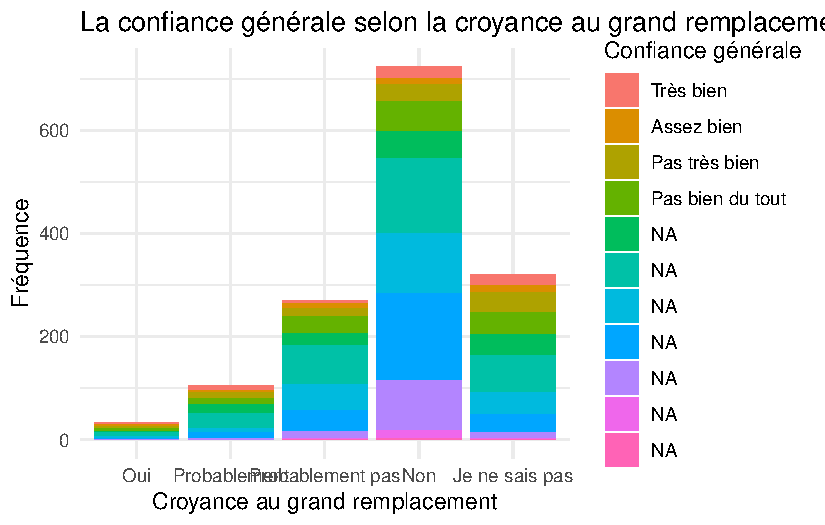
\includegraphics{travail_session_Akyildiz_files/figure-pdf/unnamed-chunk-7-1.pdf}

}

\end{figure}

Le niveau de confiance est plus haut plus le nombre est haut. Encore une
fois, notre hypothèse semble juste. Les personnes qui détiennent cette
croyance ont moins confiance aux autres. Le nombre est très élevé chez
ceux qui sont certains de l\textquotesingle existence de la théorie de
complot, et la médiane est en dessous de ceux qui sont soit douteux ou
n\textquotesingle y croient pas du tout. La médiane pour ceux qui
croient que potentiellement la théorie est vraie est la même, mais leur
nombre est plus bas. Ceux qui n\textquotesingle y croient pas du tout
sont ceux qui font le plus confiance aux autres. Ceci fait du sens. Le
grand remplacement est au final une théorie xénophobe qui nécessite un
certain niveau d\textquotesingle aliénation et de méfiance envers la
société et les gens autour d\textquotesingle eux (Goodliffe 2012). Une
plus grande méfiance indique aussi une moins grande chance de parler et
de converser avec les autres, ce qui peut mener à une aliénation encore
plus élevée et crescendo (Goodliffe 2012).

\begin{Shaded}
\begin{Highlighting}[]
\FunctionTok{ggplot}\NormalTok{(data\_super\_nettoye2, }\FunctionTok{aes}\NormalTok{(}\AttributeTok{x =} \FunctionTok{factor}\NormalTok{(Remplacement), }\AttributeTok{fill =} \FunctionTok{factor}\NormalTok{(Fonctionnement\_de\_la\_democratie))) }\SpecialCharTok{+}
  \FunctionTok{geom\_bar}\NormalTok{(}\AttributeTok{position =} \StringTok{"stack"}\NormalTok{) }\SpecialCharTok{+}
  \FunctionTok{labs}\NormalTok{(}\AttributeTok{x =} \StringTok{"Croyance au grand remplacement"}\NormalTok{, }\AttributeTok{y =} \StringTok{"Fréquence"}\NormalTok{, }\AttributeTok{fill =} \StringTok{"Fonctionnement de la démocratie"}\NormalTok{, }\AttributeTok{title =} \StringTok{"La confiance générale selon la vision du fonctionnement de la démocratie"}\NormalTok{) }\SpecialCharTok{+}
  \FunctionTok{scale\_x\_discrete}\NormalTok{(}\AttributeTok{labels =} \FunctionTok{c}\NormalTok{(}\StringTok{"Oui"}\NormalTok{, }\StringTok{"Probablement"}\NormalTok{, }\StringTok{"Probablement pas"}\NormalTok{, }\StringTok{"Non"}\NormalTok{, }\StringTok{"Je ne sais pas"}\NormalTok{)) }\SpecialCharTok{+}
  \FunctionTok{scale\_fill\_discrete}\NormalTok{(}\AttributeTok{labels =} \FunctionTok{c}\NormalTok{(}\StringTok{"Très bien"}\NormalTok{, }\StringTok{"Assez bien"}\NormalTok{, }\StringTok{"Pas très bien"}\NormalTok{, }\StringTok{"Pas bien du tout"}\NormalTok{)) }\SpecialCharTok{+}
  \FunctionTok{theme\_minimal}\NormalTok{()}
\end{Highlighting}
\end{Shaded}

\begin{figure}[H]

{\centering 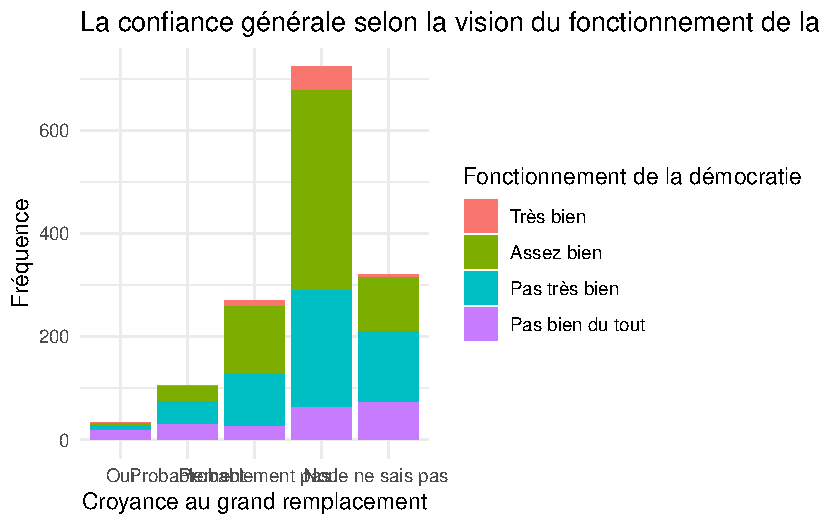
\includegraphics{travail_session_Akyildiz_files/figure-pdf/unnamed-chunk-8-1.pdf}

}

\end{figure}

Dans ce graphique à barre empilée, nous avons les différentes
appréciations de la démocratie selon les niveaux de croyance au grand
remplacement. Nous pouvons constater dès le début que
proportionnellement parlant ceux qui y croient ont quasi-unanimement une
vision négative du fonctionnement de la démocratie. Ceux qui pensent que
probablement que la théorie est vraie sont eux aussi en majorité peu
enthousiastes tandis que ceux qui n\textquotesingle y croient pas ou
presque pas sont beaucoup moins pessimistes. Ceci va encore dans le sens
de notre hypothèse, il y a une corrélation clairement visible dans ce
graphique. Pourquoi est-ce que quelqu\textquotesingle un croyant en une
théorie dont les élites vont contre les intérêts du peuple national
serait optimiste face à la démocratie? Il y a un profond mépris du
système actuel dans la pensée complotiste du grand remplacement, et ce
graphique ne fait que nous le mettre au clair (Ivaldi 2014).

\hypertarget{conclusion}{%
\subsection{Conclusion}\label{conclusion}}

En conclusion, nos résultats confirment largement nos hypothèses. Les
électeurs d\textquotesingle extrême droite sont plus méfiants des
autres, moins bien nantis, et ont une mauvaise opinion de la démocratie
française. Il y a une légère majorité d\textquotesingle homme
proportionnellement parlant qui en font partie. Nous avons confirmé cela
par notre variable fétiche, le grand remplacement qui est bien le gospel
de ces mouvements en Europe (Ivaldi 2014). Toutefois, notre pensée
qu\textquotesingle il y avait une plus grande divergence au sein de la
droite ne s\textquotesingle est pas avérée si vrai, les électeurs
semblent-ils été très similaires quant à leurs opinions sur le grand
remplacement pour ces deux partis. Ceux qui votent Zemmour ou Le Pen ont
pratiquement le même niveau de croyance et au même nombre. Il faudrait
une autre étude qui comparerait la base électorale de ces deux partis.
Au final, nos présuppositions ont été confirmé à la fois par nos
observations et par la littérature scientifique de ce sujet des plus
inquiétants mais intéressants.

\hypertarget{bibliographie}{%
\subsubsection{Bibliographie}\label{bibliographie}}

Amengay, Abdelkarim, Anja Durovic, et Nonna Mayer. 2017. «
L\textquotesingle impact du genre sur le vote Marine Le Pen ». Revue
française de science politique 67 (6): 1067-87.
https://doi.org/10.3917/rfsp.676.1067.

Goodliffe, Gabriel. 2012. «~Globalization, Class Crisis and the Extreme
Right in France in the New Century~». In \emph{Varieties of Right-Wing
Extremism in Europe}. Routledge.

Ivaldi, Gilles. 2014. «~Euroscepticisme, populisme, droites radicales~:
état des forces et enjeux européens~». \emph{L\textquotesingle Europe en
Formation} 373 (3): 7‑28. \url{https://doi.org/10.3917/eufor.373.0007}.

Quinchon-Caudal, Anne. 2021. «~Où commence
"l\textquotesingle extrême"~?~» \emph{Matériaux pour
l\textquotesingle histoire de notre temps} 139‑142 (1‑4): 3‑7.
\url{https://doi.org/10.3917/mate.139.0003}.

Todd, Emmanuel. 2021. \emph{Où en sont-elles~? Une esquisse de
l\textquotesingle histoire des femmes}. Paris: Seuil.
\url{https://www.cairn.info/revue-recherches-familiales-2023-1-page-255.htm}.



\end{document}
